\section{Absolute model differences between CAM and WACCM}\label{app_modeldiff}
The absolute temperature differences between CAM and WACCM for Reference, Control and SAI 2020 are shown in Figure \ref{fig:CAM_WACCM}. The 2-meter temperature difference reveals that CAM is much warmer than WACCM on the Northern Hemisphere, with the largest difference in the Arctic where the difference exceeds 7° in Reference and SAI 2020. In contrast, CAM is slightly cooler in the Southern Hemisphere, with the difference being generally less than 2°C except for a few areas in Reference.

This difference is lesser in Control, but still a clear difference between the two hemispheres is visible. The difference is worsened in SAI 2020, with the Arctic warming much more in CAM than in WACCM. 

As for precipitation, there is a small difference in Reference, with cam being slighly wetter over the tropics and dryer over the western Pacific Ocean. Differences shift in Control, with most notably a stark increase in precipitation over the eastern Pacific Ocean in CAM compared to WACCM. The same is seen in SAI 2020, with the ITCZ also shifting more clearly southward in CAM compared to WACCM. 

\begin{figure}[H]
	\centering
	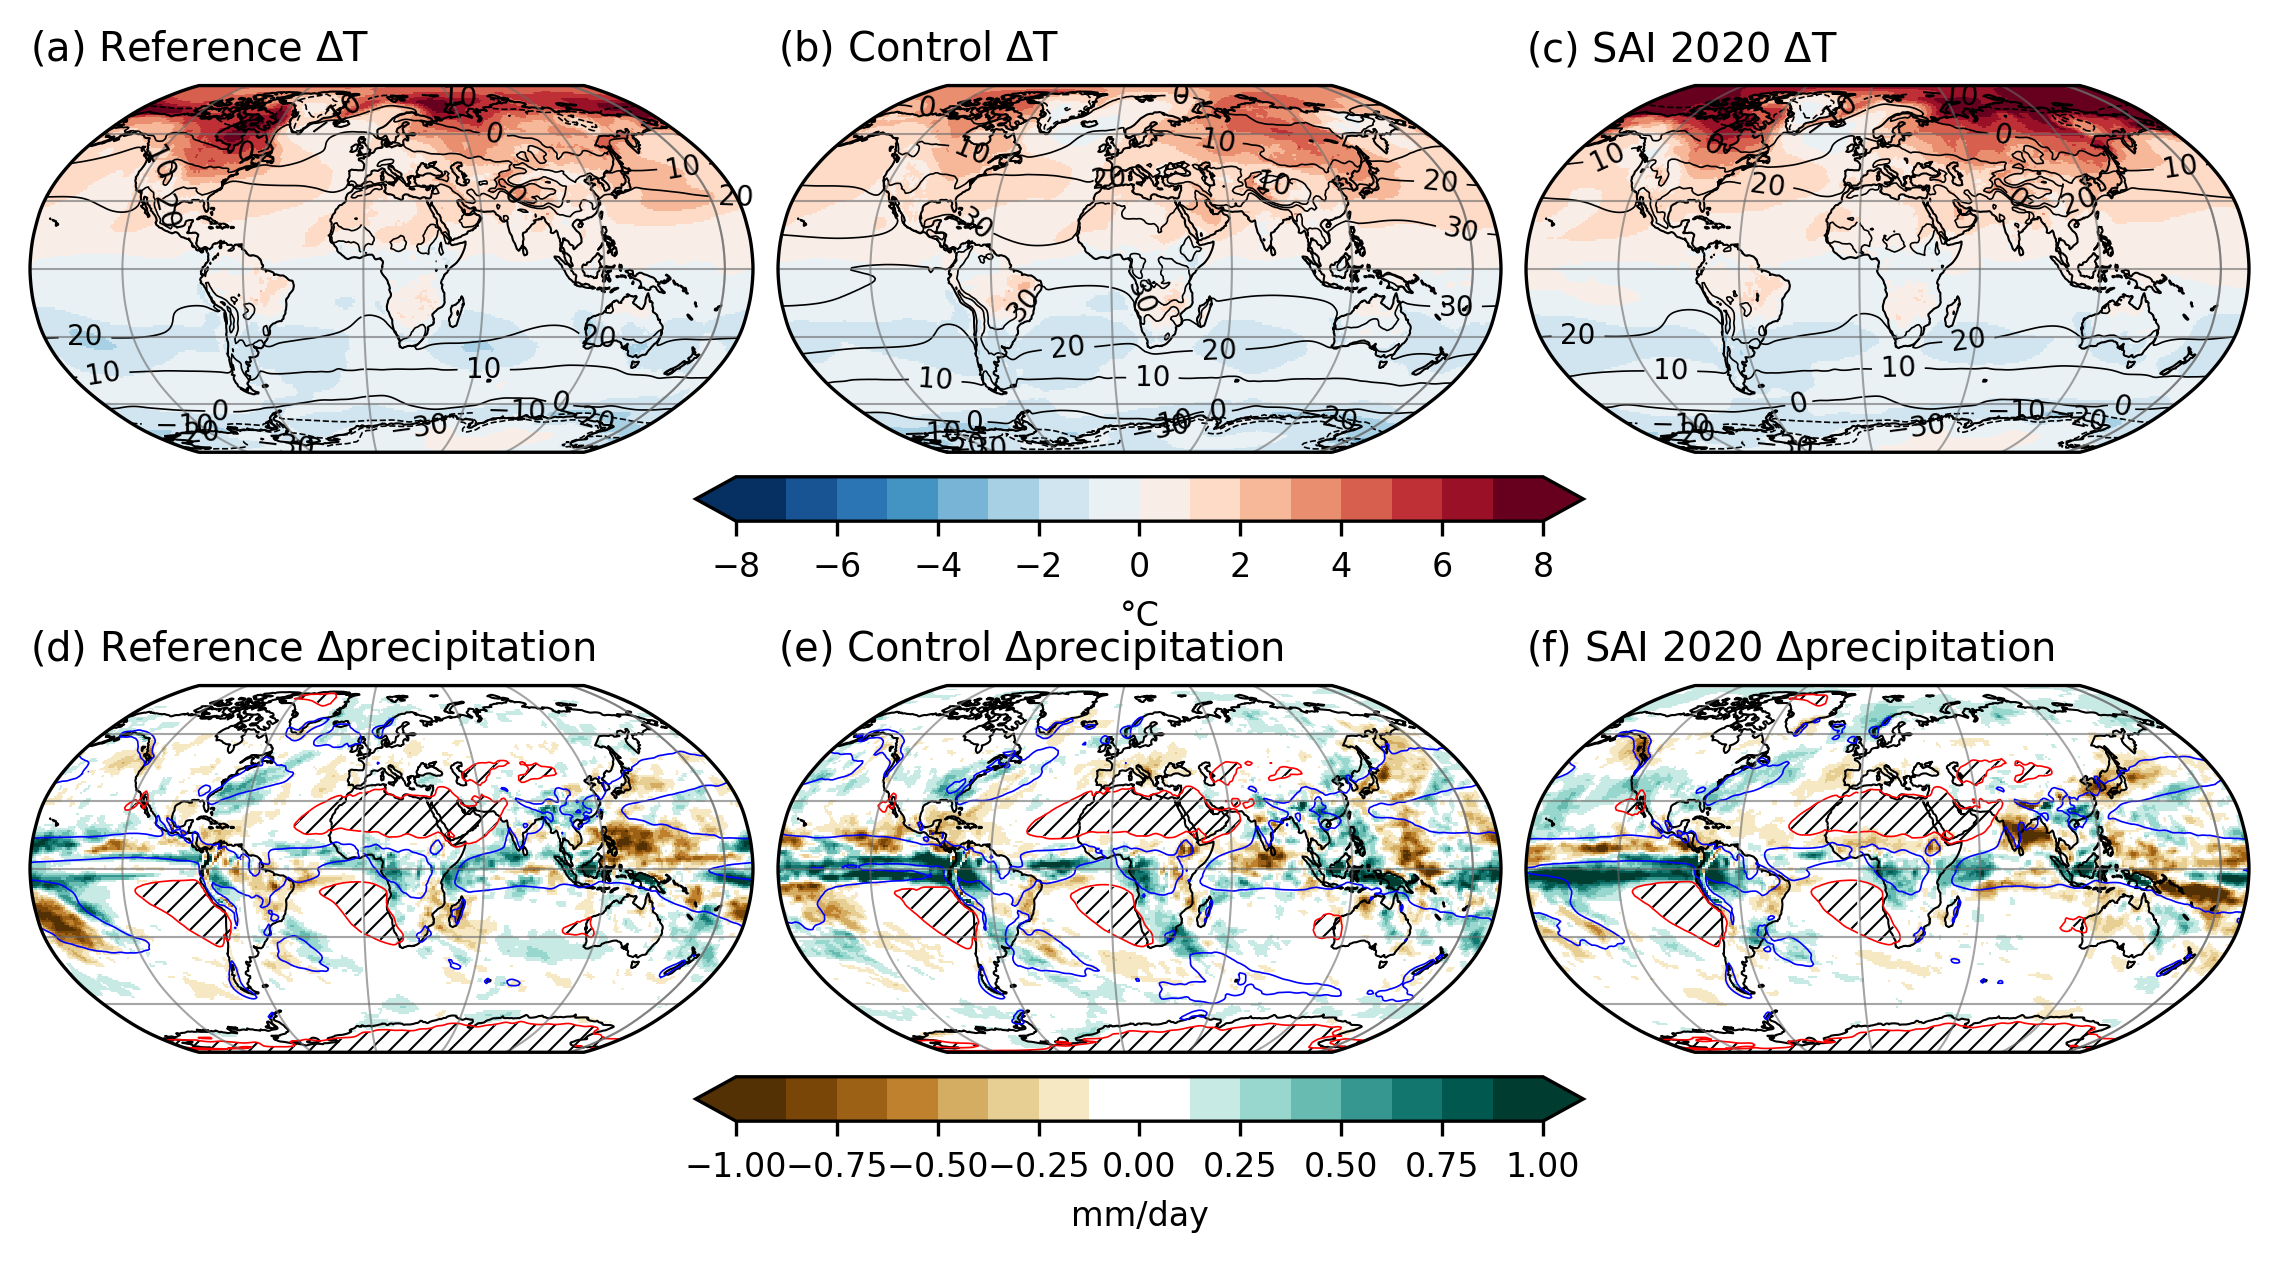
\includegraphics[width=0.95\linewidth]{images/CAM_WACCM.png}
	\caption{(a-c): Reference, Control and SAI 2020 CAM-WACCM 2-meter temperature differences, WACCM temperature in black contours in 10°C intervals; (d-e): Analogous to (a-c) for precipitation, 4 mm/day in blue contours, $<0.3$ mm/day in red contours with hatching.}
	\label{fig:CAM_WACCM}
\end{figure}

\section{Potential Temperature and Zonal Wind JJA}\label{app_th_U_JJA}

\begin{figure}[H]
	\centering
	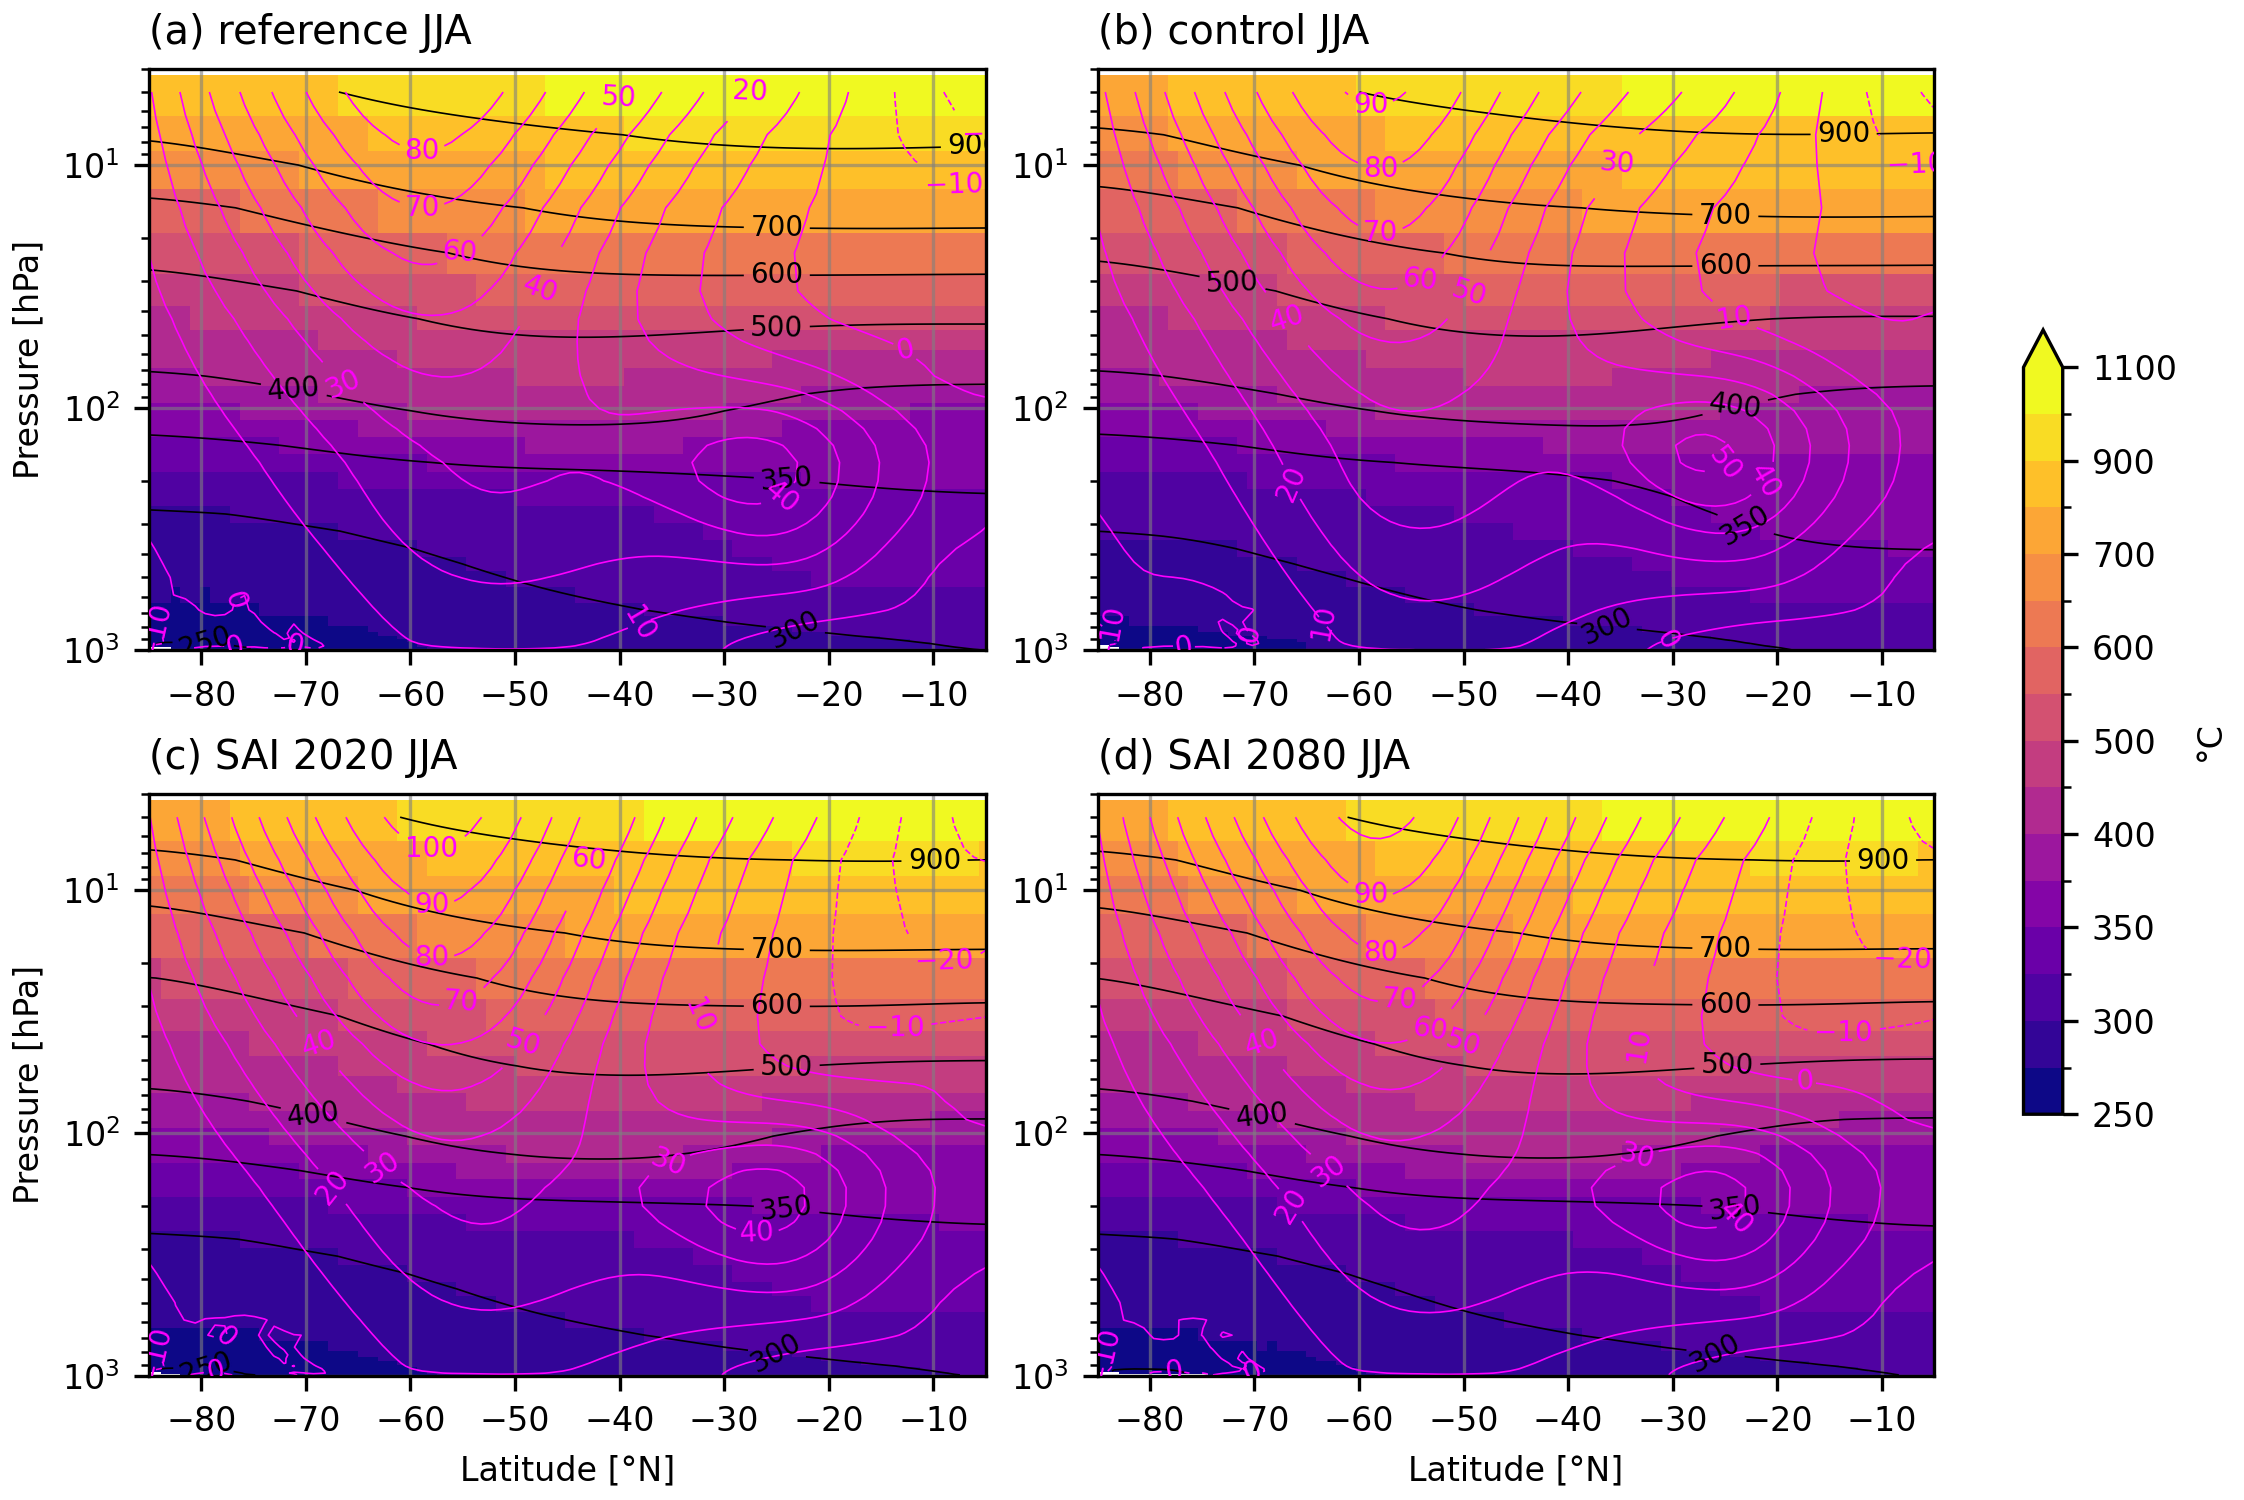
\includegraphics[width=0.95\linewidth]{images/th_U_zm_JJA.png}
	\caption{JJA mean zonal-mean potential temperature (shading and magenta contours) and zonal-mean zonal wind (black contours, m/s) for (a) Reference, (b) Control, (c) SAI 2020 and (d) SAI 2080.}
	\label{fig:th_U_zm_JJA}
\end{figure}